%% Creator: Inkscape inkscape 0.91, www.inkscape.org
%% PDF/EPS/PS + LaTeX output extension by Johan Engelen, 2010
%% Accompanies image file 'eigenfunctions.pdf' (pdf, eps, ps)
%%
%% To include the image in your LaTeX document, write
%%   \input{<filename>.pdf_tex}
%%  instead of
%%   \includegraphics{<filename>.pdf}
%% To scale the image, write
%%   \def\svgwidth{<desired width>}
%%   \input{<filename>.pdf_tex}
%%  instead of
%%   \includegraphics[width=<desired width>]{<filename>.pdf}
%%
%% Images with a different path to the parent latex file can
%% be accessed with the `import' package (which may need to be
%% installed) using
%%   \usepackage{import}
%% in the preamble, and then including the image with
%%   \import{<path to file>}{<filename>.pdf_tex}
%% Alternatively, one can specify
%%   \graphicspath{{<path to file>/}}
%% 
%% For more information, please see info/svg-inkscape on CTAN:
%%   http://tug.ctan.org/tex-archive/info/svg-inkscape
%%
\begingroup%
  \makeatletter%
  \providecommand\color[2][]{%
    \errmessage{(Inkscape) Color is used for the text in Inkscape, but the package 'color.sty' is not loaded}%
    \renewcommand\color[2][]{}%
  }%
  \providecommand\transparent[1]{%
    \errmessage{(Inkscape) Transparency is used (non-zero) for the text in Inkscape, but the package 'transparent.sty' is not loaded}%
    \renewcommand\transparent[1]{}%
  }%
  \providecommand\rotatebox[2]{#2}%
  \ifx\svgwidth\undefined%
    \setlength{\unitlength}{800bp}%
    \ifx\svgscale\undefined%
      \relax%
    \else%
      \setlength{\unitlength}{\unitlength * \real{\svgscale}}%
    \fi%
  \else%
    \setlength{\unitlength}{\svgwidth}%
  \fi%
  \global\let\svgwidth\undefined%
  \global\let\svgscale\undefined%
  \makeatother%
  \begin{picture}(1,0.75)%
    \put(0,0){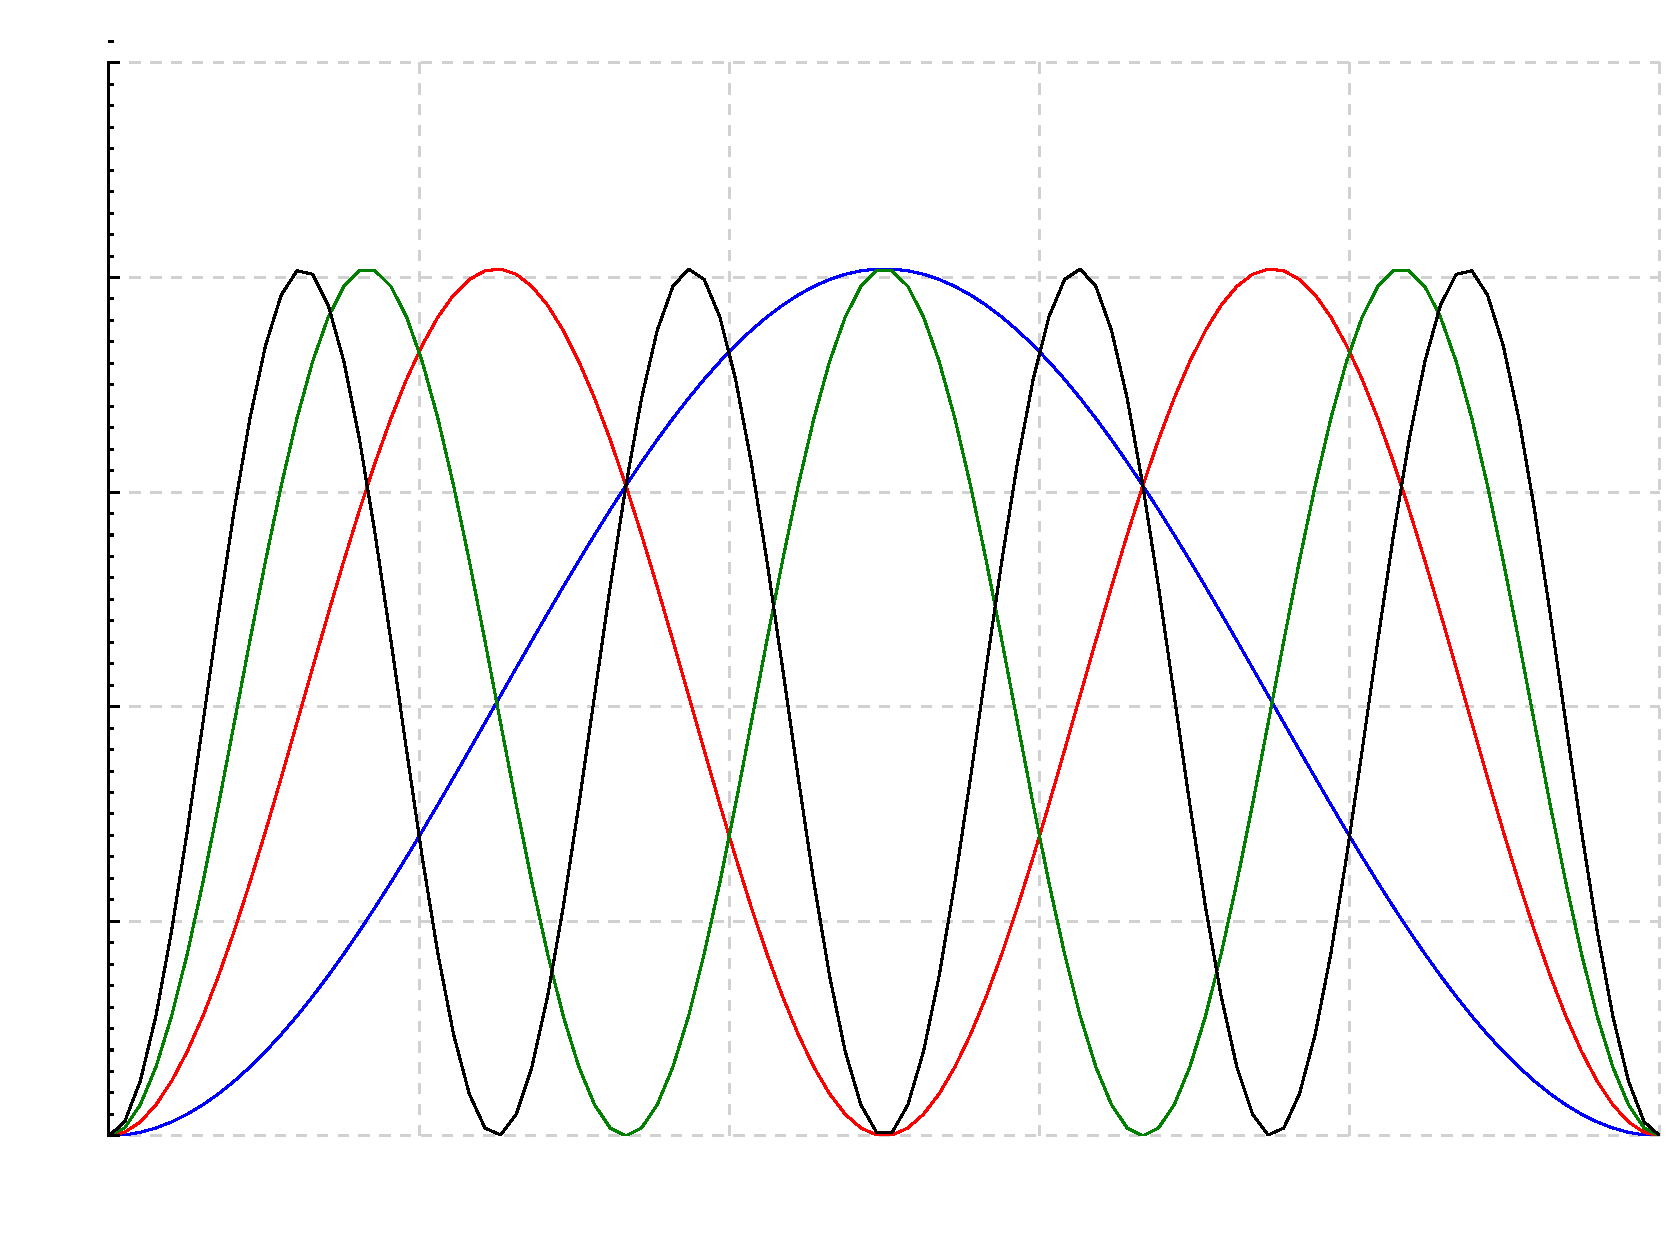
\includegraphics[width=\unitlength,page=1]{figures/eigenfunctions.pdf}}%
    \put(0.004,0.57681454){\color[rgb]{0,0,0}\makebox(0,0)[lb]{\smash{$0.02$}}}%
    \put(0,0){\includegraphics[width=\unitlength,page=2]{figures/eigenfunctions.pdf}}%
    \put(0.0,0.44990405){\color[rgb]{0,0,0}\makebox(0,0)[lb]{\smash{$0.015$}}}%
    \put(0.004,0.32290405){\color[rgb]{0,0,0}\makebox(0,0)[lb]{\smash{$0.01$}}}%
    \put(0.0,0.70690405){\color[rgb]{0,0,0}\makebox(0,0)[lb]{\smash{$0.025$}}}%
    \put(0.004,0.06340405){\color[rgb]{0,0,0}\makebox(0,0)[lb]{\smash{$0$}}}%
    \put(0.004,0.19197949){\color[rgb]{0,0,0}\makebox(0,0)[lb]{\smash{$0.05$}}}%
    \put(0.03773901,0.04840405){\color[rgb]{0,0,0}\makebox(0,0)[lb]{\smash{$0$}}}%
    \put(0.23223901,0.04){\color[rgb]{0,0,0}\makebox(0,0)[lb]{\smash{$0.2$}}}%
    \put(0.41073901,0.03){\color[rgb]{0,0,0}\makebox(0,0)[lb]{\smash{$0.4$}}}%
    \put(0.59823901,0.03){\color[rgb]{0,0,0}\makebox(0,0)[lb]{\smash{$0.6$}}}%
    \put(0.783239,0.03){\color[rgb]{0,0,0}\makebox(0,0)[lb]{\smash{$0.8$}}}%
    \put(0.970739,0.03){\color[rgb]{0,0,0}\makebox(0,0)[lb]{\smash{$1$}}}%
    \put(0.04823902,0.02040406){\color[rgb]{0,0,0}\makebox(0,0)[lb]{\smash{$\psi_1$}}}%
    \put(0.13614134,0.0200705){\color[rgb]{0,0,0}\makebox(0,0)[lb]{\smash{$\psi_2$}}}%
    \put(0.21064144,0.02057045){\color[rgb]{0,0,0}\makebox(0,0)[lb]{\smash{$\psi_3$}}}%
    \put(0.29614145,0.01957047){\color[rgb]{0,0,0}\makebox(0,0)[lb]{\smash{$\psi_4$}}}%
    \put(0.4752763,0.73714841){\color[rgb]{0,0,0}\makebox(0,0)[lb]{\smash{Eigenfunctions}}}%
  \end{picture}%
\endgroup%
